\section{Auswertung}
\label{sec:auswertung}

Im Folgenden soll eine Auswertung der aufgenommenen Messwerte erfolgen.

% \clearpage
\subsection{Phasenabhängigkeit des Ausgangssignals}
\label{sec:auswertung:phasenabhaengigkeit}

In \autoref{tab:mess_phasenabhaengigkeit} sind die Messwerte zur Phasenabhängigkeit des Ausgangssignals aufgelistet.
Die Spannungen sind als Peak-to-Peak-Beträge zu verstehen.

\begin{table}[H]
  \centering
  \caption{Messwerte zur Phasenabhängigkeit des Ausgangssignals.}
  \label{tab:mess_phasenabhaengigkeit}
  \begin{tabular}{S S[table-format=2.1] S}
    \toprule
    {$\phi \mathbin{/} \si{\degree}$} &
    {$U \mathbin{/} \si{\volt}$} &
    {$U_\text{noise} \mathbin{/} \si{\milli\volt}$} \\
    \midrule
      0 & 13.8 & 880 \\
     45 & 13.2 & 880 \\
     90 & 12.0 & 688 \\
    135 & 14.0 & 656 \\
    180 & 14.6 & 904 \\
    225 & 18.0 & 928 \\
    270 & 12.4 & 744 \\
    315 & 13.4 & 584 \\
    360 & 18.4 & 872 \\
    \bottomrule
  \end{tabular}
\end{table}

Die Abbildungen \ref{fig:screenshots_1} und \ref{fig:screenshots_2} zeigen einige Spannungsverläufe
zu den in \autoref{tab:mess_phasenabhaengigkeit} aufgelisteten Werten.

\begin{figure}
  \centering
\begin{tabular}{cc}
  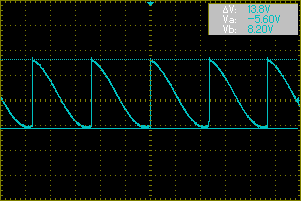
\includegraphics[width=0.45\textwidth]{content/img/screenshots/MAP003.png} &  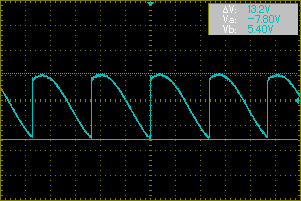
\includegraphics[width=0.45\textwidth]{content/img/screenshots/MAP008.png} \\
  $\phi = \SI{0}{\degree}$ &
  $\phi = \SI{45}{\degree}$ \\[2em]
  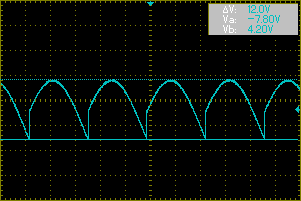
\includegraphics[width=0.45\textwidth]{content/img/screenshots/MAP005.png} &  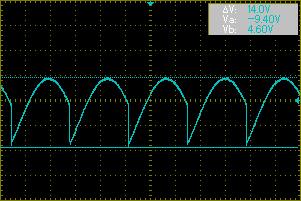
\includegraphics[width=0.45\textwidth]{content/img/screenshots/MAP010.png} \\
  $\phi = \SI{90}{\degree}$ &
  $\phi = \SI{135}{\degree}$ \\[2em]
  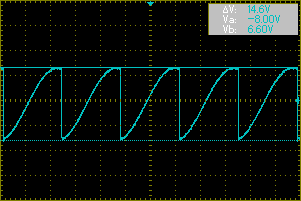
\includegraphics[width=0.45\textwidth]{content/img/screenshots/MAP004.png} &  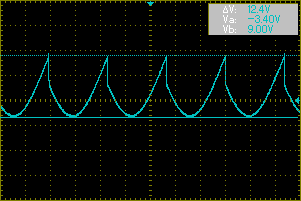
\includegraphics[width=0.45\textwidth]{content/img/screenshots/MAP006.png} \\
  $\phi = \SI{180}{\degree}$ &
  $\phi = \SI{270}{\degree}$
\end{tabular}
\caption{Screenshots des Spannungsverlaufs ohne Rausch-Generator.}
\label{fig:screenshots_1}
\end{figure}

\begin{figure}
  \centering
\begin{tabular}{cc}
  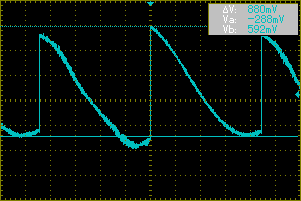
\includegraphics[width=0.45\textwidth]{content/img/screenshots/MAP013.png} &  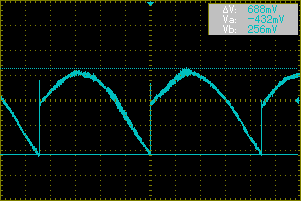
\includegraphics[width=0.45\textwidth]{content/img/screenshots/MAP014.png} \\
  $\phi = \SI{0}{\degree}$ &
  $\phi = \SI{90}{\degree}$ \\
\multicolumn{2}{c}{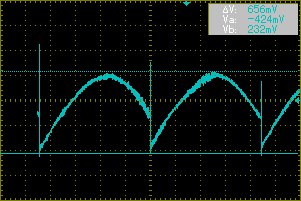
\includegraphics[width=0.45\textwidth]{content/img/screenshots/MAP015.png}} \\
\multicolumn{2}{c}{$\phi = \SI{135}{\degree}$}
\end{tabular}
\caption{Screenshots des Spannungsverlaufs mit Rausch-Generator.}
\label{fig:screenshots_2}
\end{figure}

\FloatBarrier

Die gewonnenen Werte werden nun mittels eines Fits
mit \autoref{eqn:ausgangsspannung_phase} verglichen.
Dazu wird \texttt{scipy.curve\_fit} verwendet.
Da $U$ nur betragsweise gemessen wurde,
wird auch für die Theoriekurve der Betrag verwendet.
Das Vorzeichen hätte auch gemäß $\operatorname{sgn}({\cos{(\phi)}})$ gewählt werden können,
worauf aufgrund der schlechten Datenlage (s.u.) aber verzichtet wurde.

Für das nicht verrauschte Signal (\autoref{fig:plot_phasen})
ergibt sich eine Spannung von $U_0 = \SI{29(5)}{\volt}$.

Für das verrauschte Signal (\autoref{fig:plot_phasen_noise})
ergibt sich eine Spannung von $U_0 = \SI{1.61(28)}{\volt}$.

Es zeigt sich,
dass die gemessenen Werte eher schlecht zur Theorie passen.
Dies wird in der \hyperref[sec:diskussion]{Diskussion} weiter erörtert.

\begin{figure}
    \centering
    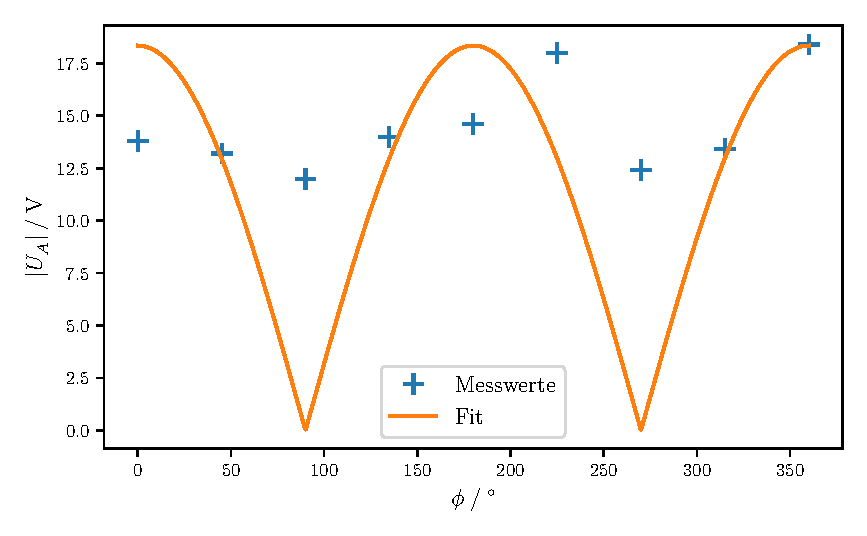
\includegraphics[width=\textwidth]{build/plt/phasen.pdf}
    \caption{Betrag der Peak-to-Peak-Spannung in Abhängigkeit von der eingestellten Phasendifferenz (klar).}
    \label{fig:plot_phasen}
\end{figure}

\begin{figure}
    \centering
    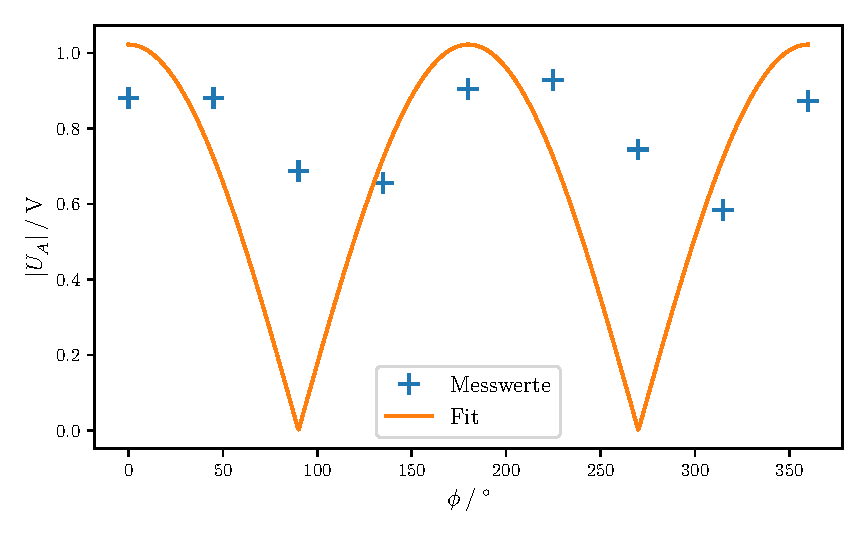
\includegraphics[width=\textwidth]{build/plt/phasen_noise.pdf}
    \caption{Betrag der Peak-to-Peak-Spannung in Abhängigkeit von der eingestellten Phasendifferenz (verrauscht).}
    \label{fig:plot_phasen_noise}
\end{figure}

\clearpage
\subsection{Rauschunterdrückung des Lock-In-Verstärkers bei einer Photodetektorschaltung}

In \autoref{tab:mess_led} sind die Messwerte für diesen Teil der Auswertung aufgeführt.
Es ist zu beachten, dass keine präzisen absoluten Distanzen,
sondern lediglich Distanz-\textbf{Unterschiede} betrachtet werden.
Die Photodiode befindet sich auf der optischen Bank bei konstant $\SI{5}{\centi\meter}$,
während konstruktionsbedingt die kleinste Position der Leuchtdiode bei $\SI{9.6}{\centi\meter}$ liegt.
Damit ergibt sich eine ungefähre Minimaldistanz von $\SI{4.6}{\centi\meter}$,
welche bereits in der \hyperref[sec:durchfuehrung:led]{Durchführung} erwähnt wurde.
In der Tabelle sind die abgelesenen Werte aufgeführt,
während für die nachfolgende Analyse die Werte so verschoben wurden,
dass sie bei 0 beginnen.

\begin{table}[H]
  \centering
  \caption{Messwerte zur Spannungsamplitude an der Photodiode in Abhängigkeit der (relativen) Distanz zur Leuchtdiode.}
  \label{tab:mess_led}
  \begin{tabular}{S[table-format=2.1] S[table-format=2.2]}
    \toprule
    {$d \mathbin{/} \si{\centi\meter}$} &
    {$U \mathbin{/} \si{\volt}$} \\
    \midrule
    \expandableinput{build/tab/led.tex}
    \bottomrule
  \end{tabular}
\end{table}

Es kann vermutet werden,
dass die einfallende Intensität und damit die gemessene Spannung
invers proportional zum Abstand oder dem Quadrat desselben ist.
Um diese Vermutung zu überprüfen,
wurden entsprechende Fits berechnet.
In \autoref{fig:plot_led} sind diese dargestellt.

Tatsächlich fällt die Intensität offenbar quadratisch mit der Distanz ab.
Für den zugehörigen Fit
\[ U = \frac{U_0}{(d + d_0)^2} \]
ergeben sich die Parameter
\begin{align*}
  U_0 &= \SI{3.07(16)e3}{\square\centi\meter\volt} \\
  d_0 &= \SI{9.61(29)}{\centi\meter}
\end{align*}
Der Parameter $d_0$ ist dabei notwenig,
weil es die Apparatur – wie zuvor erwähnt – nicht erlaubt,
Leuchtdiode und Photodiode direkt voreinander zu platzieren.
% Er entspricht überraschend genau der minimalen Position der Leuchtdiode,
% was aber Zufall sein muss,
% weil für den Fit die Position der Leuchtdiode als 0 angenommen wurde.
% Es sollte also idealerweise 4.6 rauskommen.

\begin{figure}
  \centering
  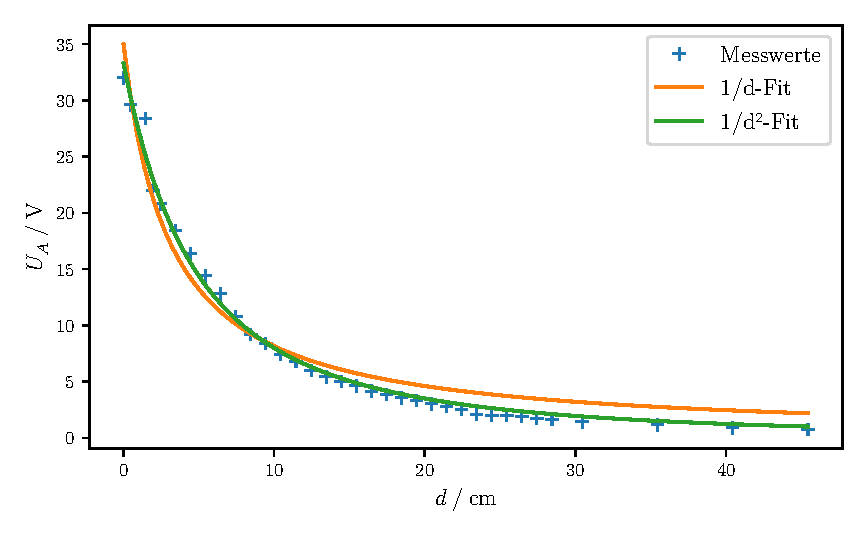
\includegraphics[width=\textwidth]{build/plt/led.pdf}
  \caption{Spannungsamplitude an der Photodiode in Abhängigkeit der (relativen) Distanz zur Leuchtdiode.}
  \label{fig:plot_led}
\end{figure}
